\chapter{Questionnaire Text}
\label{Appendix:Questionaire_text}

Note: This questionnaire was presented on Survey Monkey and thus the text here is a best approximation of their paging system.


\section*{Page 1 - Introduction}

Thank you for taking part in this research.

According to Survey Monkey, this survey should take 6 minutes to complete, when we tested it, the average was closer to 10 minutes.

This survey is for the validation section of a research master's project by Paul Spencer at the University of Amsterdam.

The purpose is to determine whether projectional editing can be used to aid the comprehensibility of business rules.

We are using Drools as our example business rules language.

You were selected as you asked or answered a Drools question on StackOverflow, listed Drools as a skill on your LinkedIn profile, or were referred to this survey by someone who previously answered this survey.
(please feel free to forward this survey to anyone you know with Drools experience).

It is therefore assumed you are aware of what Drools is.

Projectional editing is a form of writing computer programs directly rather than writing text and having that parsed to create the program.
This allows the developer multiple views and editors for the same code.

In this survey, we will present you with a few of these views.

On the following page, there is an animated GIF that will give a small demonstration of what this means.

Figure \ref{fig:questionnaire_intro} shows how this is presented to the subject.

\section*{Page 2 - Example of Projectional editing in Drools}

Below is an animated GIF showing an example of a projectional implementation of Drools.

The top section is a tabular projection of the program.

The bottom part is a textual projection of the same program shown at the same time.

In this recording, we are editing in the tabular projection, which automatically updates the textual projection.

\emph{\underline{Here is placed an animated GIF of a demonstration of our prototype}}

\textbf{Question}: What is your first reaction to this mode of code editing?

Options: Very positive, Somewhat positive, Neutral, Somewhat negative, Very negative 

\emph{\underline{the order of the options will be randomly presented as either ``Very positive'' to ``Very negative'' or ``Very negative'' to ``Very positive''}}

Figure \ref{fig:questionnaire_firstImpression} shows how this is presented to the subject.

\section*{Page 3 - Positive about projectional editing}

\emph{\underline{This page is only selected if the user chose very positive or somewhat positive}}

This question is optional.

you may use the Green ``PREV'' button to review the previous page.

\textbf{Question}: how would this coding style be useful to your interactions with Drools?

This is an open question with a text box.

Figure \ref{fig:questionnaire_positive} shows how this is presented to the subject.

\section*{Page 4 - negative about projections}

\emph{\underline{This page is only selected if the user chose very positive or somewhat positive}}

This question is optional.

you may use the Green ``PREV'' button to review the previous page.

\textbf{Question}: What do you find negative with this style of coding

This is an open question with a text box.

\section*{Page 5 - Testing a projection}
\emph{\underline{In questionnaire version A \& D page 5 will be Testing a projection}}

\emph{\underline{In questionnaire version B \& C page 5 will be Testing textual projection}}

On this page, we present you with an example projection of a collection of Drools rules, in this case, as a sort of decision table.

We will ask you to describe what you think it does, if you can't that is also good data for us.

A brief description of how this projection works follows:

\emph{\underline{for the decision table the following text:}}

1) each row is a rule

2) each column is a fact, or, when indented, a selection criteria of that fact

3) smiley faces indicate that a fact has been selected for a rule

4) if a fact has been selected and a variable is bound to it then the variable name appears instead of the smiley face.

5) the ``Then'' part of the rule appears in the ``Actions'' column

\emph{\underline{for the other table the following text:}}

1) each row is a rule

2) each column is for a variable or a property of a fact

3) if a property is selected then the selection criteria is in the appropriate cell

4) unselected cells are indicated by a grey/beige colour

5) the ``Then'' part of the rule appears in the ``Actions'' column


\emph{\underline{depending on the version of this questionnaire the respondent will see one of the following pictures}}

\emph{\underline{Version A - decision table showing rule set 1 (FNWI)}}

\emph{\underline{Version B - decision table showing rule set 2 (LAW)}}

\emph{\underline{Version C - new table showing rule set 1}}

\emph{\underline{Version D - new table showing rule set 2}}

\textbf{Question}: Please describe what you think this group of rules does

This is an open question with a text box.

\textbf{Question}: How easy or difficult was it to describe this rule set?

Options: Very easy, Somewhat easy, Neutral, Somewhat difficult, Very difficult 

\emph{\underline{the order of the options will be randomly presented as either ``Very easy'' to ``Very difficult'' or ``Very difficult'' to ``Very easy''}}

Figure \ref{fig:questionnaire_describeProjection} shows how this is presented to the subject.

\section*{Page 6 - Testing textual projection}
\emph{\underline{In questionnaire version A \& D page 6 will be Testing textual projection}}

\emph{\underline{In questionnaire version B \& C page 6 will be Testing a projection}}

Here we present you a textual projection of Drools rules.

[Note: These are not the same rules as on the previous page]

\emph{\underline{depending on the version of this questionnaire the respondent will see one of the following pictures}}

\emph{\underline{Version A \& C - a text projection of rule set 2 (LAW)}}

\emph{\underline{Version B \& D - a text projection of rule set 1 (FNWI)}}

\textbf{Question}: Please describe what you think this group of rules does

This is an open question with a text box.

\textbf{Question}: How easy or difficult was it to describe this rule set?

Options: Very easy, Somewhat easy, Neutral, Somewhat difficult, Very difficult 

\emph{\underline{the order of the options will be randomly presented as either ``Very easy'' to ``Very difficult'' or ``Very difficult'' to ``Very easy''}}

Figure \ref{fig:questionnaire_describeText} shows how this is presented to the subject.

\section*{Page 7 - Comparing projections 1}

In this question, we ask to compare a new projection to a previously shown projection, on the page named ``Testing a projection''.

If you wish to reacquaint yourself with the previous projection, you can use the Green ``PREV''  button at the bottom of this page.

A brief description of how this new projection works follows:

\emph{\underline{for the decision table the following text:}}

1) each row is a rule

2) each column is a fact, or, when indented, a selection criteria of that fact

3) smiley faces indicate that a fact has been selected for a rule

4) if a fact has been selected and a variable is bound to it then the variable name appears instead of the smiley face.

5) the ``Then'' part of the rule appears in the ``Actions'' column


\emph{\underline{for the other table the following text:}}

1) each row is a rule

2) each column is for a variable or a property of a fact

3) if a property is selected then the selection criteria is in the appropriate cell

4) unselected cells are indicated by a grey/beige colour

5) the ``Then'' part of the rule appears in the ``Actions'' column

\emph{\underline{depending on the version of this questionnaire the respondent will see one of the following pictures}}

\emph{\underline{Version A - new table showing rule set 1}}

\emph{\underline{Version B - new table showing rule set 2}}

\emph{\underline{Version C - decision table showing rule set 1}}

\emph{\underline{Version D - decision table showing rule set 2}}

\textbf{Question}: How does the above projection compare to the first projection you described?

Options: Much easier to understand, Somewhat easier to understand, Neutral, Somewhat harder to understand, Much harder to understand

\emph{\underline{the order of the options will be randomly presented as either ``Much easier to understand'' to ``Much harder to understand'' or ``Much harder to understand'' to ``Much easier to understand'' }}

Figure \ref{fig:questionnaire_compareProjections} shows how this is presented to the subject.

\section*{Page 8 - Comparing projections 2}

In this question, we again ask to compare the new projection, this time to the textual projection, on the page named ``Testing textual projection''.

If you wish to reacquaint yourself with the textual projection, you can, of course, use the Green ``PREV'' button at the bottom of this page again.

\emph{\underline{depending on the version of this questionnaire the respondent will see one of the following pictures}}

\emph{\underline{Version A - new table showing rule set 2}}

\emph{\underline{Version B - new table showing rule set 1}}

\emph{\underline{Version C - decision table showing rule set 2}}

\emph{\underline{Version D - decision table showing rule set 1}}

\textbf{Question}: How does the above projection compare to the text Drools rules you described?

Options: Much easier to understand, Somewhat easier to understand, Neutral, Somewhat harder to understand, Much harder to understand

\emph{\underline{the order of the options will be randomly presented as either ``Much easier to understand'' to ``Much harder to understand'' or ``Much harder to understand'' to ``Much easier to understand'' }}

Figure \ref{fig:questionnaire_compareWithText} shows how this is presented to the subject.

\section*{Page 9 - Single rule helper 1 - Truth table}
\emph{\underline{In questionnaire version A \& D page 9 will be the Truth Table}}

\emph{\underline{In questionnaire version B \& C page 9 will be the Circuit Diagram}}

Below we present another projection.
This is a truth table projection.
It highlights the conditions that have to be true for a rule to be selected.

The GIF shows the rule selected and the developer pressing the up and down arrow keys to step through the different true (highlighted in green)  and false (highlighted in red) fact selections that result in a true outcome.

\emph{\underline{An animated GIF of the truth table example}}

\textbf{Question}: Would this help you with understanding your Drools rules?

Options: It would really help understanding, it would somewhat help understanding, Neutral, It would add a little confusion, It would add a lot of confusion

\emph{\underline{the order of the options will be randomly presented as either ``It would really help understanding'' to ``It would add a lot of confusion'' or ``It would add a lot of confusion'' to ``It would really help understanding''}}

Figure \ref{fig:questionnaire_truthTable} shows how this is presented to the subject.

\section*{Page 10 - Single rule helper 2 - Circuit Diagram}
\emph{\underline{In questionnaire version A \& D page 10 will be the Circuit Diagram}}

\emph{\underline{In questionnaire version B \& C page 10 will be the Truth Table}}

This is a circuit diagram of the selection conditions.
choosing a different condition highlights how they are related to each other.

The GIF shows the rule selected and the developer pressing the up and down arrow keys to step through the different fact selections (highlighted in yellow) and shown in the circuit diagram, thus showing how the facts relate to each other.

\emph{\underline{An animated GIF of the Circuit Diagram example}}

\textbf{Question}: Would this help you with understanding your Drools rules?

Options: It would really help understanding, it would somewhat help understanding, Neutral, It would add a little confusion, It would add a lot of confusion

\emph{\underline{the order of the options will be randomly presented as either ``It would really help understanding'' to ``It would add a lot of confusion'' or ``It would add a lot of confusion'' to ``It would really help understanding''}}

Figure \ref{fig:questionnaire_circuitDiagram} shows how this is presented to the subject.

\section*{Page 11 - The Statistics page}
Here we ask for data that we can use to slice and dice results.

\textbf{Question}: How long was/is your career as a developer?

Options: 0-1 year, 1-3 years, 3-10 years, greater than 10 years, none of the above

\textbf{Question}: When was the last time you had a coding interaction with Drools?

Options: during this week, some time after July 1st 2021, some time after Jan 1st 2021, some time after 2016, some time before 2016

\textbf{Question}: how long did you work with Drools?

Options: for years and intensely, for years but occasionally, not for long but intensely, I barely touched it


\textbf{Question}: Which tools have you used to edit Drools rules?

Checkboxes: Drools workbench, eclipse (with Drools plug-in), IntelliJ IDEA (with Drools plug-in), IDE or text editor without Drools assistance, other (please specify) \emph{\underline{has textbox}}, none of the above

Figure \ref{fig:questionnaire_personalDetails} shows how this is presented to the subject.

\section*{Page 12 - So long, and thanks for all the fish}
Thank you for your time.
We leave you with a box where you can put in any thoughts about this if you feel like it.

\textbf{Question}: Do you have any thoughts or opinions you would like to share about what you have seen in this questionnaire?

This is an open question with a text box.

Figure \ref{fig:questionnaire_comments} shows how this is presented to the subject.

\begin{figure}
    \centering
    \fbox{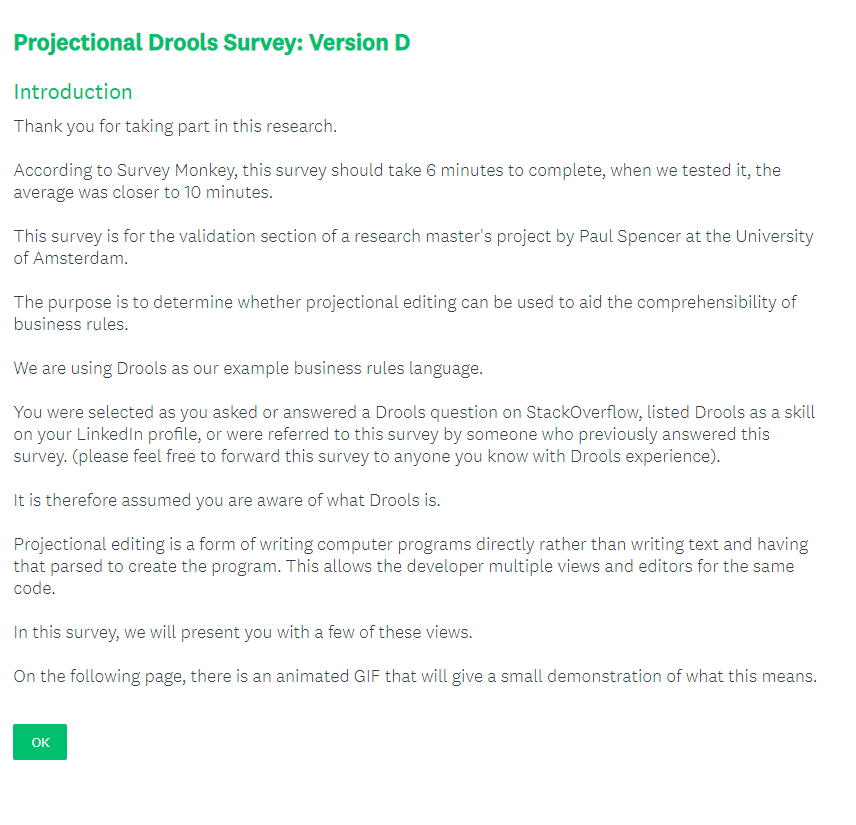
\includegraphics[width=0.95\textwidth]{Appendices/images/questionnaire_1.png}}
    \caption{Screen 1 - introduction text}
    \label{fig:questionnaire_intro}
\end{figure}
 
\begin{figure}
    \centering
    \fbox{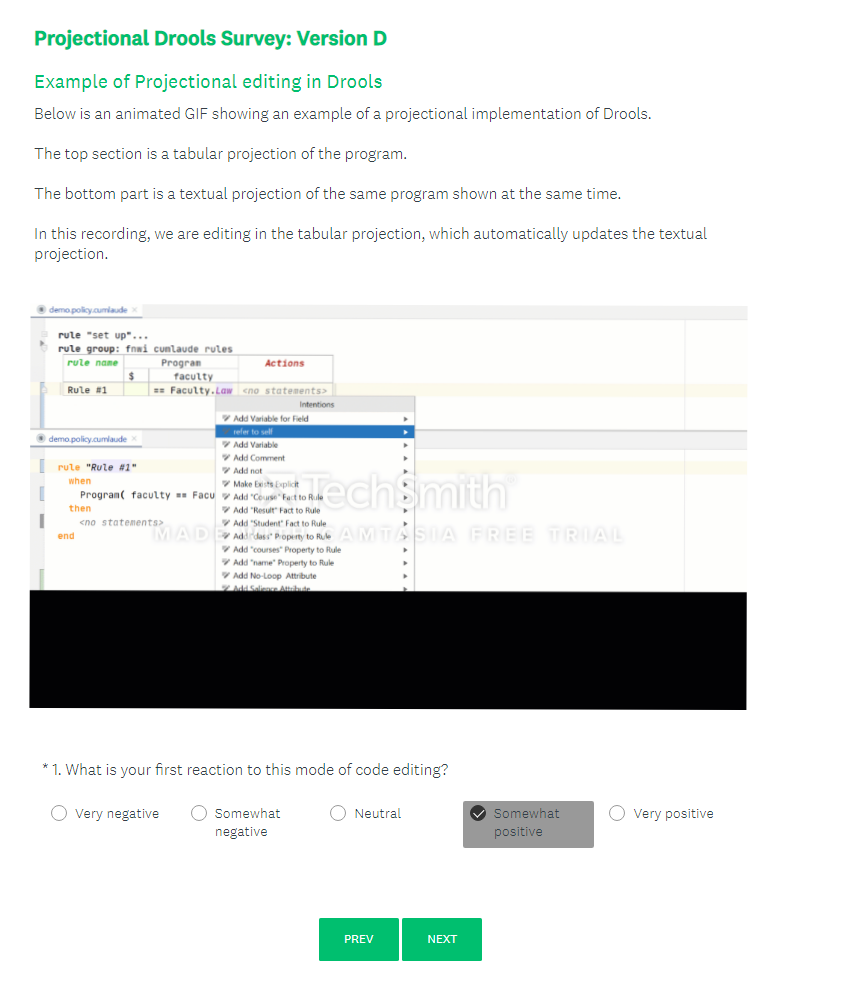
\includegraphics[width=0.95\textwidth]{Appendices/images/questionnaire_2.png}}
    \caption{Screen 2 - first impression}
    \label{fig:questionnaire_firstImpression}
\end{figure}
 
\begin{figure}
    \centering
    \fbox{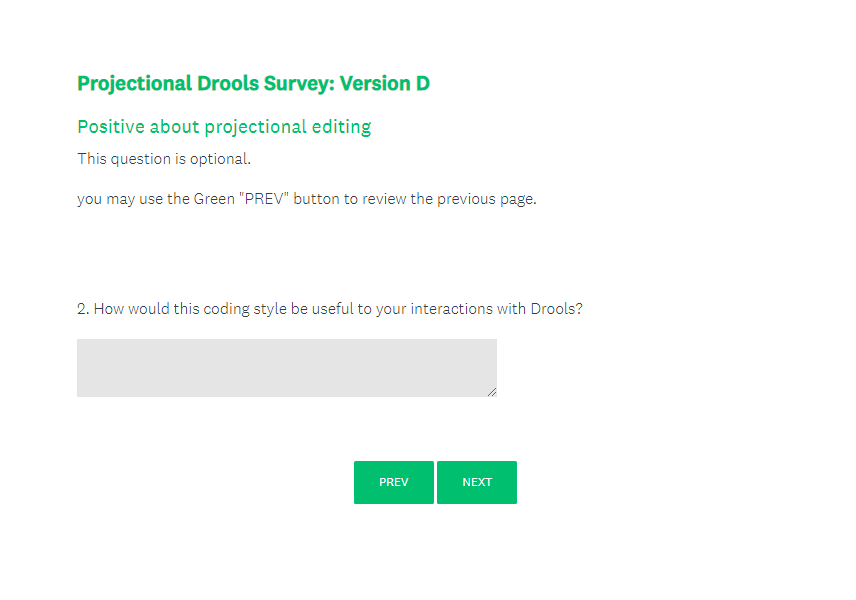
\includegraphics[width=0.95\textwidth]{Appendices/images/questionnaire_3.png}}
    \caption{Screen 3 - positive response}
    \label{fig:questionnaire_positive}
\end{figure}
 
\begin{figure}
    \centering
    \fbox{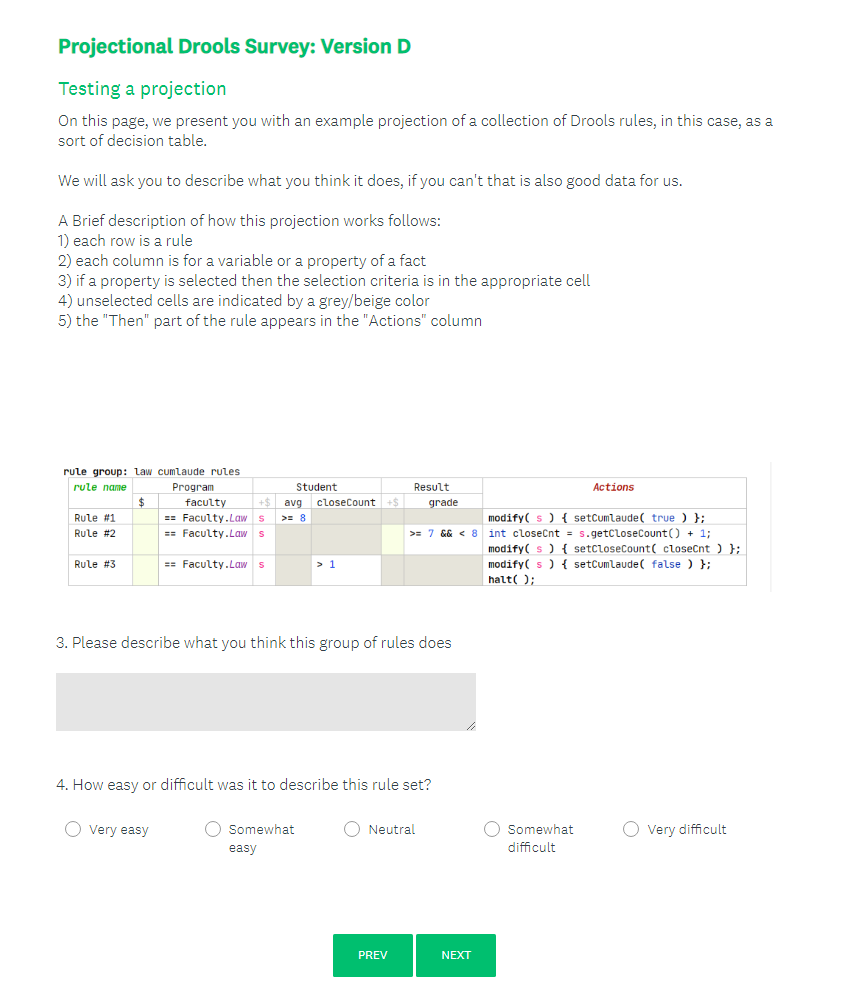
\includegraphics[width=0.95\textwidth]{Appendices/images/questionnaire_4.png}}
    \caption{Screen 4 - describe projection}
    \label{fig:questionnaire_describeProjection}
\end{figure}
 
\begin{figure}
    \centering
    \fbox{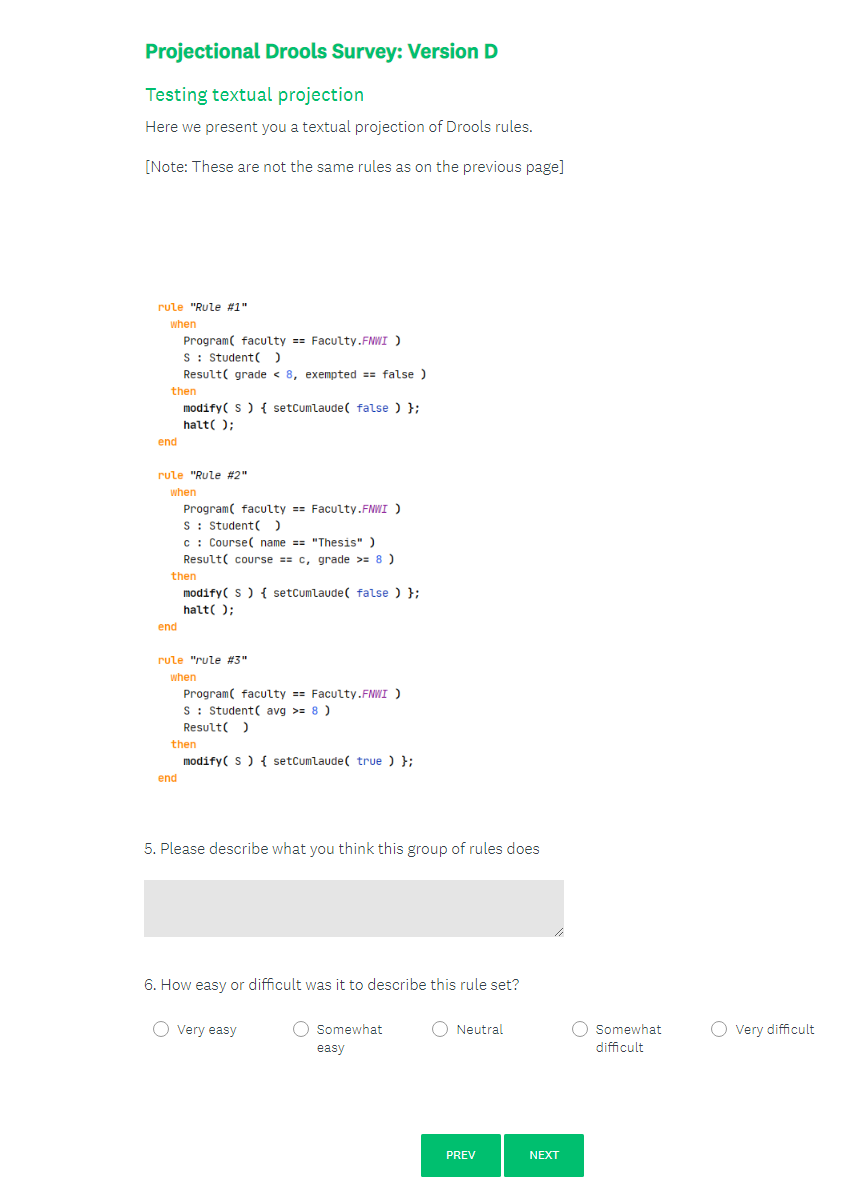
\includegraphics[width=0.95\textwidth]{Appendices/images/questionnaire_5.png}}
    \caption{Screen 5 - describe text}
    \label{fig:questionnaire_describeText}
\end{figure}
 
\begin{figure}
    \centering
    \fbox{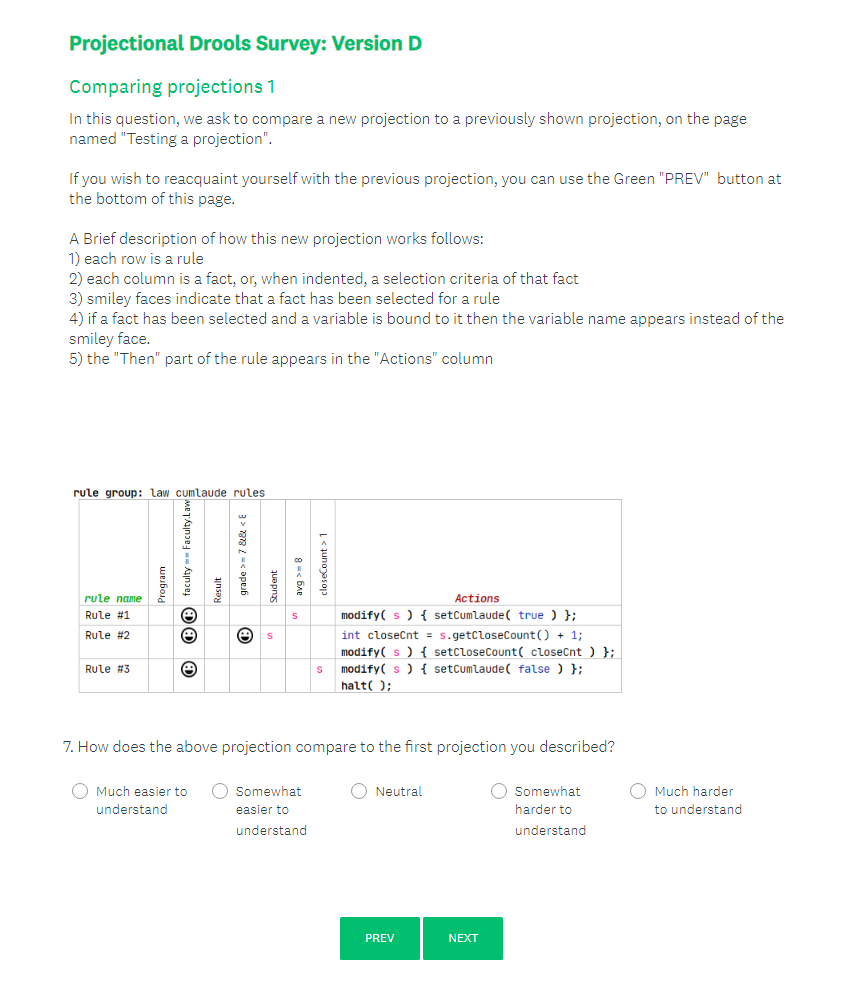
\includegraphics[width=0.95\textwidth]{Appendices/images/questionnaire_6.png}}
    \caption{Screen 6 - compare projections}
    \label{fig:questionnaire_compareProjections}
\end{figure}
 
\begin{figure}
    \centering
    \fbox{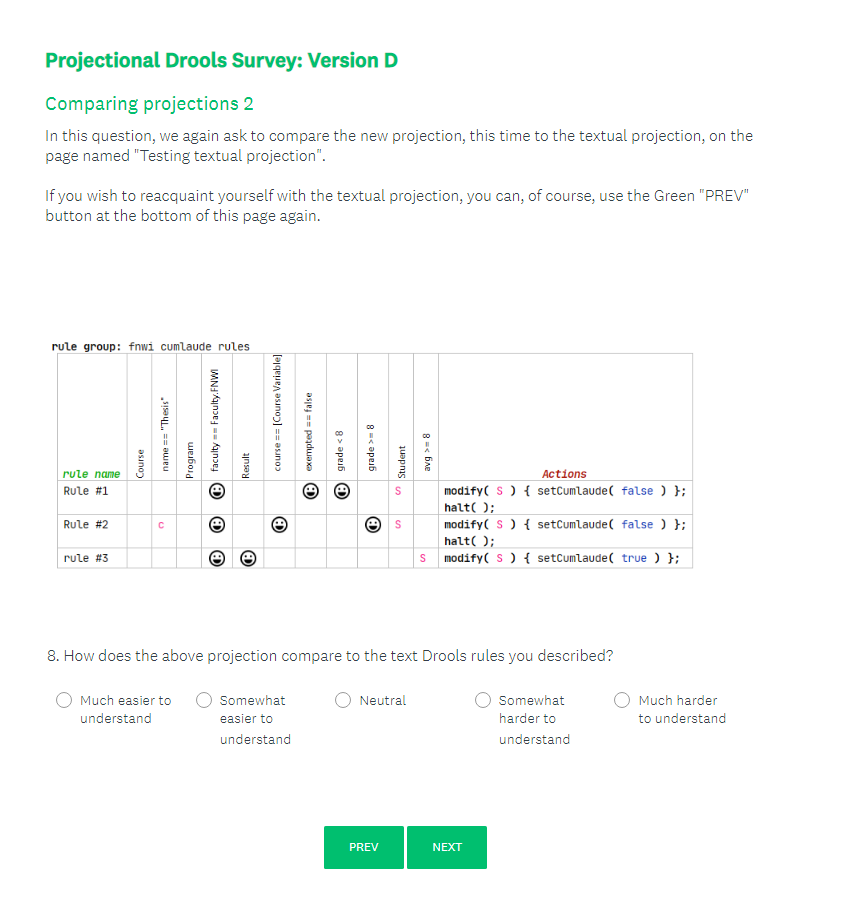
\includegraphics[width=0.95\textwidth]{Appendices/images/questionnaire_7.png}}
    \caption{Screen 7 - compare projection to text}
    \label{fig:questionnaire_compareWithText}
\end{figure}
 
\begin{figure}
    \centering
    \fbox{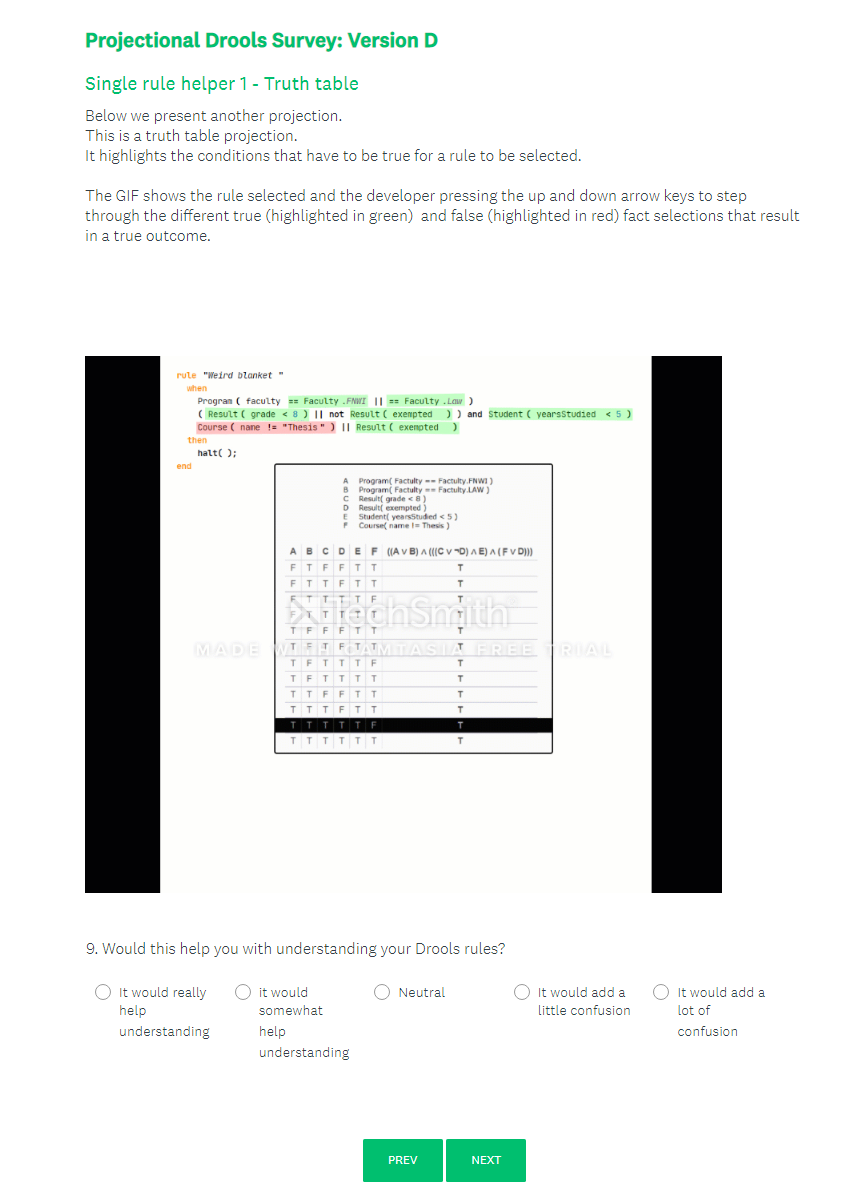
\includegraphics[width=0.95\textwidth]{Appendices/images/questionnaire_8.png}}
    \caption{Screen 8 - truth table}
    \label{fig:questionnaire_truthTable}
\end{figure}
  
\begin{figure}
    \centering
    \fbox{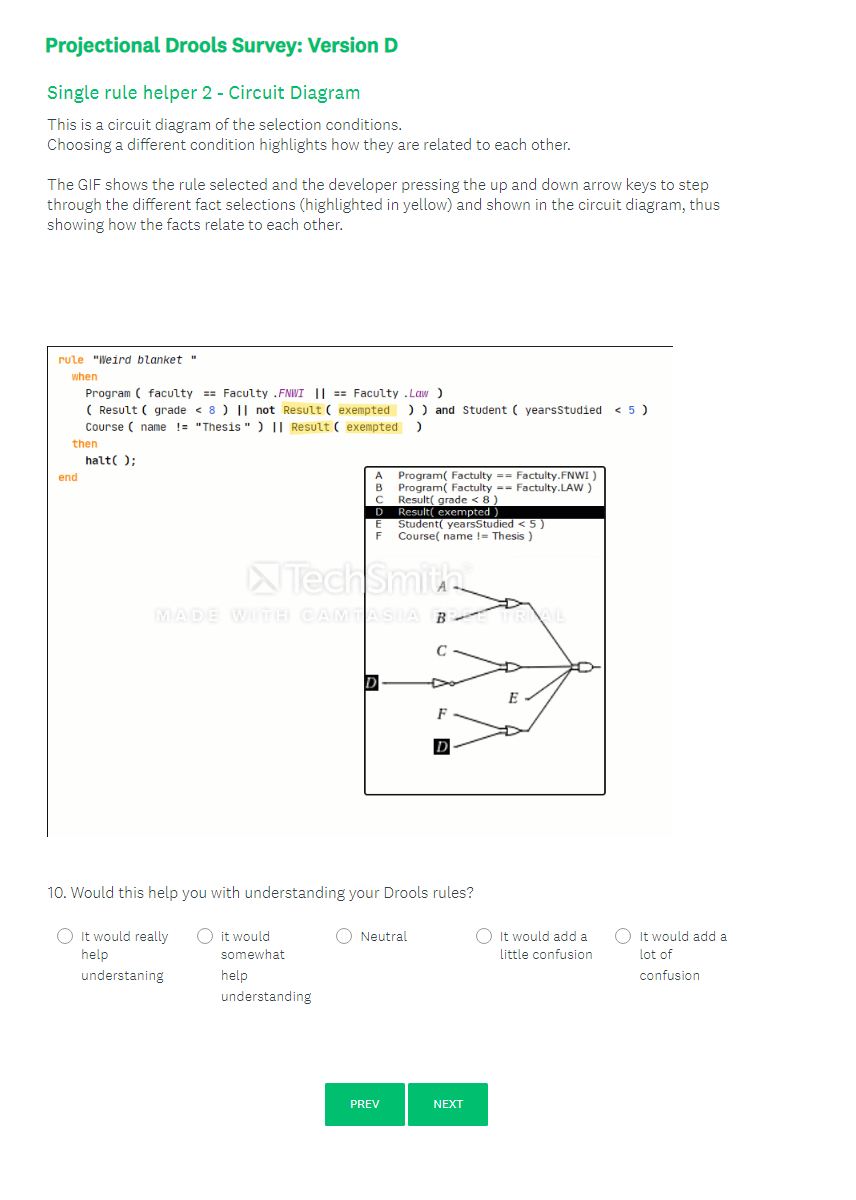
\includegraphics[width=0.95\textwidth]{Appendices/images/questionnaire_9.png}}
    \caption{Screen 9 - circuit diagram}
    \label{fig:questionnaire_circuitDiagram}
\end{figure}
   
\begin{figure}
    \centering
    \fbox{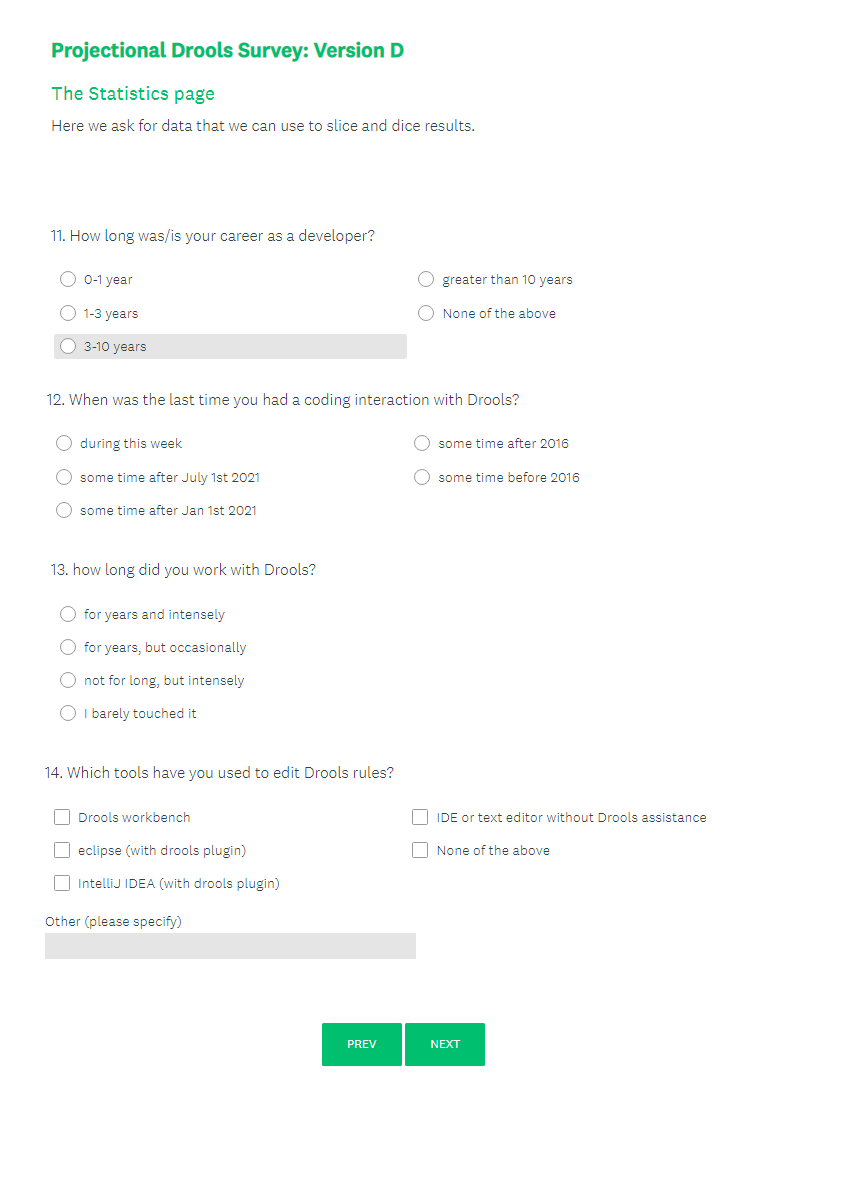
\includegraphics[width=0.95\textwidth]{Appendices/images/questionnaire_10.png}}
    \caption{Screen 10 - personal details page}
    \label{fig:questionnaire_personalDetails}
\end{figure}
   
\begin{figure}
    \centering
    \fbox{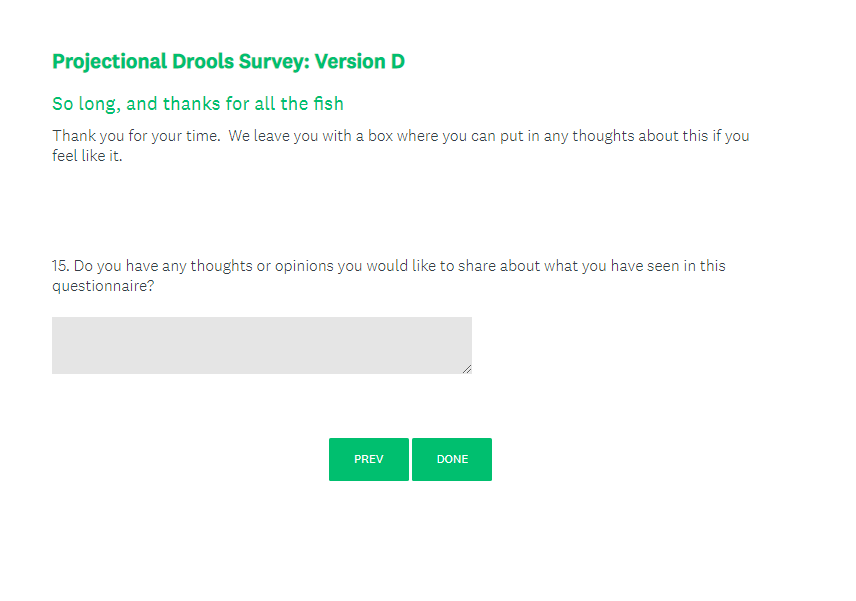
\includegraphics[width=0.95\textwidth]{Appendices/images/questionnaire_11.png}}
    \caption{Screen 11 - further comments}
    \label{fig:questionnaire_comments}
\end{figure}